\chapter{Código Limpo}
\label{chap:codigo_limpo}

A definição de um bom código não é precisa ou exata. Do mesmo modo que enfretamos dificuldades para definir o que é arte, não podemos definir um conjunto de parâmetros lógicos e mensuráveis para delimitar a diferença de qualidade entre códigos-fonte. Podemos considerar aspectos como testabilidade, eficiência, facilidade de modificação, processo pelo o qual foi desenvolvido, entre outros. Portanto, no âmbito deste trabalho, nos deteremos a trabalhar com o chamado código limpo orientado a objetos.

No livro \textit{Clean Code} \citep{Martin2008}, o autor entrevistou grandes especialistas em desenvolvimento de software como Ward Cunningham (inventor de \textit{Fit}, \textit{Wiki} e \textit{Programação Extrema} \citep{Beck1999}) e Dave Thomas (fundador da OTI e muito envolvido no Projeto Eclipse) questionando-os quanto a uma definição para código limpo. Cada um dos entrevistados elaborou respostas diferentes, destacando características subjetivas, como elegância, facilidade de alteração e simplicidade, e outras puramente técnicas, incluindo a falta de duplicações, presença de testes unitários e de aceitação e a minimização do número de entidades.

Em certo sentido, um código limpo está inserido em um estilo de programação que busca a proximidade para com três valores: expressividade, simplicidade e flexibilidade. Tais termos são utilizados por Kent Beck no livro Implementation Patterns \citep{Beck2007} que estão em conforme com a unidade de pensamento que permeia as respostas dos especialistas.

\subsubsection{Expressividade}
Dentre as definições encontradas pela pesquisa de Robert Martin acima citada, algumas afirmações se destacam quanto a expressividade. Na visão de Grady Booch \citep{Booch2007}, um código limpo pode ser lido como um texto em prosa e deixa claro as intenções do autor através de operações e abstrações bem escolhidas. Já para Dave Thomas e Kent Beck, a medida para a expressividade está na facilidade para um desenvolvedor, que não o autor original do trecho de código, entender, modificar e utilizá-lo.

Grande parte dessas ideias receberam influência do livro de Donald Knuth, \textit{Literate Programming} \citep{Knuth92}. A intenção era programar em linguagens naturais, como o inglês e português, e intercalar as expressões com macros e pequenos trechos de código-fonte tradicional. O arquivo poderia ser lido como um texto comum, mas no plano de fundo seriam executados os trechos correspondentes à cada uma das expressões em linguagem natural.

Nesse sentido, um código é expressivo quando pode ser facilmente lido nas diferentes camadas de abstração, deixando detalhes de implementação ``escondidos'' em níveis mais baixos. Nas palavras de Ward Cunningham, a solução implementada faz com que a linguagem pareça ter sido feita para o problema sendo resolvido.

\subsubsection{Simplicidade}
A simplicidade é um dos aspectos mais valorizados por Kent Beck. Na sua visão, devemos programar buscando reduzir a quantidade de informação que o leitor deve compreender para fazer alterações. Desta maneira, o autor dá grande importância para a minimização do número de abstrações, comentários e estruturas complexas entre as classes que são desnecessários.

\subsubsection{Flexibilidade}
A flexibilidade reflete a facilidade de estender a aplicação sem fazer grandes alterações na estrutura já implementada. Não queremos ter que mudar diversos métodos e diversas classes para adicionar uma funcionalidade.

O código pretendido deve se adequar e aproveitar bem das vantagens inerentes ao paradigma da orientação a objetos. Tal adequação está bem representada tanto nos princípios \textit{SOLID} \citep{Martin2000}, quanto nos princípios apresentados em \textit{Implementation Patterns} abaixo.

\begin{itemize}
	\item Consequências Locais: devemos estruturar o código de forma que as alterações fiquem encapsuladas em partes do programa;
	\item Minimizar Duplicações: devemos particionar o programa em partes pequenas com o intuito de minimizar as repetições tanto na forma de trechos semelhantes como em hierarquias de classe parelelas e estruturas com informações duplicadas;
	\item Proximidade da Lógica e Dados: devemos aproximar a lógica e os dados sobre quais trabalha uma vez que ambos serão alterados simultaneamente;
	\item Simetria: devemos criar abstrações de maneira simétrica para que o leitor, uma vez entendida uma das partes, entenda rapidamente as demais.
\end{itemize}

\section{O Desenvolvimento de um Código Limpo} 
Um importante aspecto quanto o desenvolvimento de um código limpo é o reconhecimento que não será obtido em uma primeira tentativa. Robert Martin ressalta que as versões iniciais de um método, classe e outras estruturas nunca são exatamente uma boa solução. É necessário tempo e preocupação com cada elemento desde o nome escolhido para uma variável até uma hierarquia de classes.

Diante dessa realidade, queremos garantir que não teremos empecilhos para as refatorações.
O mais crítico dos impedimentos é a insegurança. Se ao fazer uma alteração, ficamos receosos de que algo pode ter quebrado, provavelmente logo deixaremos de fazê-las, progressivamente afastando o código da limpeza desejada. Desta forma, a presença de testes automatizados são a fundação para o desenvolvimento de um código limpo. Os testes dão a segurança de que as partes estão funcionando corretamente, possibilitando as diversas refatoracões para deixar o código claro.

Além de auxiliar nas alterações, os testes compõe parte da expressividade, simplicidade e flexibilidade de um código. Para que desenvolvedores que não o autor de um trecho de código o compreendam, os testes podem reportar como o elemento deve ser usado. Por fim, a medida para a simplicidade pode ser feita através da suíte de teste: se os testes estão todos corretos, não é necessário adicionar complexidade, apenas melhorias sem adicionar funcionalidade. 

Outro tipo de empecilho que podemos encontrar são os comentários e documentações para métodos e classes. Para qualquer alteração feita no código, em tese os comentários e formas de documentação também deveriam ser mudados para ficarem de acordo com o estado atual. Uma contraposição é muito frequente, como aponta Robert Martin: por um lado, se nos policiarmos para que a atualização do código e comentários seja simultânea, muito provavelmente deixaremos de fazer alterações devido ao excesso de trabalho; pelo outro, se deixarmos de atualizar uma das formas de documentação, estaremos tornando-as dispensáveis, além de potencialmente se tornarem fontes de informações incorretas.

A solução dada é focar a atenção no desenvolvimento de um código limpo. Se as variáveis estiverem devidamente nomeadas, não precisaremos criar um comentário para explicá-la. Se os métodos estiverem bem nomeados e tiverem uma única tarefa, não será necessário documentar o que são os parâmetros e o valor de retorno. E por fim, se os testes estiverem bem executados, teremos uma documentação do código que garante a corretude.

Robert Martin enfatiza que o desejado é não engessar o desenvolvimento e melhoria do código com dificuldades para os programadores, mas compreender quais elementos do software precisam de documentação e contruí-la adequadamente.

\vskip 1.0cm
As sessões subsequentes apresentam aspectos importantes para termos um código limpo no que diz respeito a detalhes quanto aos nomes, métodos e classes.

\section{Nomes}
\label{sec:nomes}

Em uma primeira análise sobre um código-fonte, uma das afirmações que pode ser feita é que ele é constituído por um conjunto de palavras reservadas da linguagem e um número imenso de nomes escolhidos pelos desenvolvedores. Por exemplo, um código escrito em Smalltalk praticamente não contém palavras da sintaxe da linguagem, contendo uma grande quantidade de envio de mensagens aos objetos e usos de variáveis, ambos com nomes escolhidos pelos desenvolvedores.

\subsubsection{Nomes que Revelam Intenção}
De acordo com Robert Martin, o nome de uma variável, método ou classe deveria responder todas as questões acerca do elemento sendo nomeado. Deveria contar porque o elemento existe, o que faz e como deve ser usado, de forma que comentários se tornem redundantes. O exemplo abaixo ilustra a dificuldade do leitor compreender um código com nomes pouco reveladores.

\lstinputlisting[label=nomes_pouco_reveladores, caption={Exemplo de nomes pouco reveladores}]{codigos/nomes_pouco_reveladores}

Esse método, pertencente à uma classe Grafo, é difícil de ser compreendido sem um vasto conhecimento da convenção de notações e o algoritmo utilizado. Muitas perguntas poderiam ser feitas como (i) O que faz caminhoR?,  (ii) O que é o vértice v?  E quanto ao w? Eles tem algo em comum?, (iii)  O que significa adj(v, w) ser igual a 1?.

A seguir segue o mesmo código com alterações somente nos nomes das variáveis e métodos, sem nenhuma alteração na implementação.

\lstinputlisting[label=passeio_com_origem_em, caption={Melhorias nos nomes podem tornar o código mais claro}]{codigos/passeio_com_origem_em}

Muitas questões podem ser respondidas depois da leitura desse trecho. O nome da função deixa claro que sua tarefa é passear pelos vértices do grafo começando pelo vértice origem passado como parâmetro. O vetor est foi renomeado para estado e as constante 0 e -1 receberam um nome, revelando o significado das operações em que constam. A simples mudança de \textit{tamanho()} para \textit{numeroDeVertices()} provê um contexto mais completo para o entendimento do laço.
	
O exemplo poderia ser melhorado para ficar mais alinhado com o paradigma da orientação a objetos e com os conceitos que serão apresentados mais adiante. Nesta sessão tratamos a importância da escolha de nomes e como pode auxiliar o entendimento. É possível revelar o significado de elementos dando nomes para as constantes, por exemplo. Nomes como origem e próximo podem nomear objetos da mesma classe para mostrar o contexto e semântica de como estão sendo usados. Métodos podem trazer mais expressividade e fluência à leitura se forem nomeados levando em conta o código cliente e nas circunstâncias em que será chamado.

\subsubsection{Diferenças Significativas}
Durante a criação de um método ou uma classe, é muito comum que, no mesmo contexto, haja  objetos de tipos iguais. Nessa situação, não basta escolher nomes que representem bem o que é o objeto, mas também é preciso criar uma diferença significativa entre eles. O intuito é deixar claro ao leitor do código  (i.e. programador) o papel de cada uma das partes, tanto para facilitar o uso de métodos deixando claro a ordem dos parâmetros, quanto para que a semântica de uma operação fique mais clara.
	
Quando um leitor se depara com um método como \textit{copiaElementos(lista1, lista2)}, pode não ficar claro qual é a ordem dos argumentos: os elementos da lista1 são copiados para lista2 ou vice-versa? Com uma simples distinção criada através dos nomes, a leitura não levanta nenhum tipo de dúvidas em \textit{copiaElementos(origem, destino)}.

\subsubsection{Nomes Temporários}
Uma solução utilizada para melhorar a clareza das operações de um trecho de código é utilizar nomes temporários para revelar como um objeto será utilizado naquele contexto. O exemplo abaixo ilustra bem esse tipo de situação.

\lstinputlisting[label=encontra_caminho_entre_v1, caption={Exemplo sem o uso de nomes temporários}]{codigos/encontra_caminho_entre_v1}

Com algum esforço, o leitor identificará que o código está buscando o caminho entre a estação Jabaquara e a última estação da linha Amarela. Porém, a expressividade da versão alterada abaixo deixa com que a leitura e compreensão sejam imediatas.

\lstinputlisting[label=encontra_caminho_entre_v2, caption={Usando nomes temporários}]{codigos/encontra_caminho_entre_v2}


\subsubsection{Nome Único por Conceito}
Outra recomendação dada por Robert Martin \citep{Martin2008} se refere a unicidade de nomes por conceito. O objetivo do estilo de programação buscado é facilitar a compreensão do código e nomear um conceito de maneiras diferentes é bastante confuso, uma vez que o leitor não saberá se o contexto trata de ideias distintas. Qual seria a diferença entre \textit{get}, \textit{fetch}, \textit{retrieve}? Ou encontrar, procurar e buscar?
	
Se apenas uma nomenclatura for utilizada, o leitor não terá questões, além de poder se aproveitar da simetria de operações valorizada por Kent Beck \citep{Beck2007}. Não é um acaso que os métodos sobre coleções sempre possuem um mesmo conjunto de nomes como o método \textit{add} para adicionar elementos. Desta forma, as dúvidas de qual deles utilizar para cada uma das opções é minimizada, sendo mais fácil a assimilação do conceito.

\subsubsection{Nomes dos Métodos}
Na próxima sessão serão apresentados fundamentos teóricos quanto ao uso de métodos para a documentação do código através de sua expressividade. Antes, para que as técnicas exemplificadas sejam eficazes como pretendido por Robert Martin e Kent Beck, os nomes dos métodos devem ser bem escolhidos de modo que descrevem muito bem a tarefa que realizam.
	
O uso de nomes descritivos pode muitas vezes resultar em nomes longos e difíceis de serem digitados muitas vezes. Entretanto, a quantidade de ocasiões em que serão lidos é substancialmente maior do que a quantidade em que as escrevemos. Desta maneira, a economia de palavras deve ser descartada em favor de uma boa expressividade \citep{Beck2007}.
	
A linguagem Smalltalk é constantemente elogiada quanto a sua expressividade. Grande parte dos elogios estão concentrados no uso de seletores para o envio de mensagens para os objetos. Podemos gerar métodos como \textit{criaJogoDeFutebolEntre:} SãoPaulo \textit{e:} Palmeiras \textit{naData:} data. Os elementos em itálico são o verdadeiro protótipo do método, deixando claro a ordem dos argumentos, seu papel e o que exatamente está sendo executado. Essas são as características desejadas para os nomes dos métodos formarem em conjunto uma narrativa da execução.

\section{Métodos}
\label{sec:metodos}

Os métodos são o núcleo fundamental para a criação de um código expressivo. Considerando as ideias levantadas por Grady Booch e Kent Beck, o objetivo é desenvolver um código que seja lido como um texto em prosa e, nessa analogia, a intenção é utilizar os nomes dos métodos para narrar a execução.
	
De acordo com os princípios já abordados anteriormente, buscamos minimizar as repetições e queremos que as mudanças sejam localizadas, de forma que a lógica esteja perto dos dados que manipula. Nesse sentido, os métodos encapsulam um trecho de código, provendo um escopo fechado para variáveis locais e permitindo chamadas como uma maneira de evitar duplicações.

\subsection{Fundamentação Teórica}
O primeiro fundamento levantado no livro \textit{Clean Code} quanto aos métodos é uma preocupação quanto ao tamanho. Segundo Robert Martin, métodos devem ser pequenos (e se possível menores do que isso). O autor também cita que não existe uma fundamentação científica para tal afirmação, além de não podermos afirmar o que é “pequeno” e definir limitantes quanto ao número de linhas.
	
A proposta é que cada método seja pequeno o suficiente para facilitar sua leitura e compreensão. Devemos ter em vista a dificuldade de assimilação de grandes porções de informação durante a leitura e o fato de que nem sempre uma instrução é clara. A partir dessas ideias, um método será uma porção curta de código que trabalha com poucas variáveis e tem um nome explicativo que espelha a sua funcionalidade.
	
Uma maneira bastante interessante de pensar sobre o tamanho dos métodos não é simplesmente contar seu número de linhas, mas compreender bem a tarefa que realiza. Nas palavras de R. Martin, “Funções deveriam ter uma única tarefa. Deveriam fazê-la bem. E fazê-la somente.”
	
Isso significa que para criar uma lista de números primos usando o algoritmo do \textit{Crivo de Erastótenes}, não queremos ter um único método que contenha todos os detalhes da criação de uma lista de inteiros e a marcação de múltiplos que não tem chance de serem primos. Seria muito difícil entendê-lo e modificar detalhes da implementação. Queremos várias métodos pequenos que fazem cada uma das tarefas necessárias para essa computação, de forma que a leitura seja suficiente e uma documentação externa redundante.
	
Outra questão teórica importante e enfatizada por Kent Beck são os níveis de abstrações e a simetria de operações dentro de um método. Um incremento de uma variável de instância está fundamentalmente em outro nível de abstração do que a chamada de um método. Não queremos um método com essas duas instruções. Isso possivelmente faz com que o leitor não saiba se uma operação é um detalhe de implementação ou um conceito importante dentro da lógica, além de abrir as portas para mais ocorrências deste mesmo tipo, aumentando a complexidade do código a cada alteração.
	
Pensando em outros fatores que podem levar a dificuldades para a leitura do nosso código, sabemos que estamos trabalhando em um código limpo quando cada rotina que lemos faz o que esperávamos \citep{Martin2008}. No contexto de métodos, como seus nomes são a documentação da tarefa que realizam, não queremos que, ao olhar o corpo de um deles, nos deparemos com uma operação que não imaginávamos. Ao criar um método, temos que considerar que os leitores não terão a mesma linha de pensamento que temos naquele momento e, diante disso, temos que ter uma crescente preocupação com todas as nossas decisões.
	
O último fundamento teórico quanto aos métodos também diz respeito ao programa como um todo. Queremos ter um fluxo normal bem estabelecido, deixando-o simples e o tratamento de erros separado. Em outras palavras, não queremos que o código fiquei cheio de verificações de erro misturados com a lógica sem erros.
	
\subsection{Técnicas}
Tendo em vista a fundamentação teórica, a seguir estão algumas técnicas que nos possibilitam criar métodos que se encaixem no estilo de programação buscado.

\subsubsection{Composição de Métodos}
\label{metodos:composicao}
A composição de método é a base para a criação de um código limpo. A proposta é compor nossos métodos em chamadas para outros métodos rigorosamente no mesmo nível de abstração.
	
Usando novamente o exemplo do algoritmo do \textit{Crivo de Erastótenes}, para encontrar os primos de 1 a N devemos criar um conjunto de elementos que represente os inteiros de 1 a N, marcar todos números múltiplos de outros e depois coletar todos aqueles que não estão marcados (os primos). Para isso criamos um método da classe \textit{GeradorDePrimos}:

\lstinputlisting[label=primos_ate, caption={Algoritmo do Crivo de Erastótenes decomposto em métodos}]{codigos/primos_ate}

Nesse exemplo, compusemos o método \textit{primosAte(N)} em chamadas para outros métodos, cada um com uma tarefa e um nome explicativo. Dessa forma, o leitor pode entender facilmente como funciona o algoritmo de uma maneira geral. 
	
Também ficam bastante claros os níveis de abstrações criados. A função primosAte(n) está em um nível e os métodos que invoca estão todos no mesmo patamar logo abaixo. Queremos criar essa estrutura em cadeia, tornando possível que o leitor só precise entender os níveis que interessem no momento.
	
A composição de métodos não é uma técnica que desconhecemos, uma vez que a todo momento criamos estruturas dessa maneira sem ter conhecimento da sua efetividade. Entretanto, a facilidade de leitura propiciada faz com que esse seja o padrão mais relevante do livro~\citep{Beck2007, InfoQ2010}. 	

\subsubsection{Métodos Explicativos (Explaining Methods)}
\label{metodos:explicativos}
Para auxiliar na expressividade de um trecho de código, podemos criar um método com nome específico do contexto em que será invocada. A operação pode ser bastante simples como um incremento de variável ou a chamada de um método em um objeto guardado em uma variável de instância, mas o nome dado será de grande valor para a documentação do código. Além disso, a função pode ser reutilizada posteriormente evitando duplicações e encapsulando a operação.
	
Essa ideia pode ser empregada em diferentes contextos e níveis de abstração. Para Kent Beck, devemos considerar a criação de um método explicativo quando ficamos tentados a comentar uma única linha de código. Abaixo está um exemplo em Java extraído do livro \textit{Implementation Patterns}.

\lstinputlisting[label=operacao_estranha, caption={Exemplo de operação pouco clara que recebe comentário}]{codigos/operacao_estranha}

O comentário pede uma mudança usando um método explicativo.
	
\lstinputlisting[label=metodo_explicativo, caption={Exemplo de Método Explicativo que dispensa os comentários}]{codigos/metodo_explicativo}

Em outro exemplo, criamos um método chamado \textit{destaca()} para dar o contexto necessário para uma operação de nível mais baixo. 

\lstinputlisting[label=destaca, caption={Método destaca() facilita a leitura do código cliente}]{codigos/destaca}

Considerando a região de código que chama \textit{destaca()}, as melhorias são diversas com essa alteração. Se a operação fosse simplesmente colocada sem nenhum comentário, provavelmente o leitor se perguntaria porque a cor de fundo da palavra está sendo alterada naquele contexto. O comentário seria algo como “destacar a palavra no texto”, o que se torna obsoleto com o método explicativo. 

Por fim, ainda há formas mais implícitas de utilizar métodos explicativos. Quando utilizamos o padrão de projeto Wrapper \citep{GOF95} para criar uma classe que abstrai uma coleção de elementos, estamos de uma maneira criando uma interface cujos métodos façam mais sentido para o domínio de aplicação trabalhado.

\subsubsection{Métodos como Condicionais}
\label{metodos:condicionais}
Um caso específico de método explicativo bastante utilizado é uma chamada para um método que contenha uma expressão booleana como valor de retorno.
	
\lstinputlisting[label=condicional_estranho, caption={Exemplo de uma expressão booleana pouco clara}]{codigos/condicional_estranho}

Um condicional como o mostrado acima não é muito claro e deixa o próprio autor confuso quanto ao seu significado depois de certo tempo após sua redação. A criação de uma função que contenha a expressão booleana nos permite escolher um nome apropriado para a circunstância, deixando o condicional claro.

\lstinputlisting[label=condicional_com_funcao, caption={Método que encapsula expressão booleana}]{codigos/condicional_com_funcao}

\subsubsection{Evitar Estruturas Encadeadas}
Tendo em vista a busca por métodos pequenos e com uma única tarefa, um aspecto relevante é a criação de estruturas encadeadas. Se um método tem uma cadeia de \textit{ifs} e \textit{elses}, o leitor terá dificuldades para compreender todos os casos e fluxos possíveis.
	
Em ambos os livros trabalhados, os autores enfatizam sobre o uso de chamadas de métodos logo em seguida de um condicional. Novamente a operação que será encapsulada estará dentro de um método com nome expressivo, o que deixa esse método curto e expressivo.
	
Mais uma vez utilizando o exemplo do \textit{Crivo de Eristótenes}, é necessário marcar todos os números que sejam múltiplos de um primo, representado por um número não marcado.

\lstinputlisting[label=marca_multiplos, caption={Alternativa para evitar estruturas encadeadas usando funções pequenas}]{codigos/marca_multiplos}

Cada método encapsula um nível na cadeia de estruturas encadeadas. Ao invés de muitos \textit{fors} e \textit{ifs} encadeados, obtivemos funções pequenas e muito focadas em uma única tarefa que podem ser mais facilmente testadas de forma independente.

\subsubsection{Cláusulas Guarda (Guard Clauses)}
Outra técnica para evitar o uso de estruturas complexas de condicionais são as cláusulas guarda. Quando criamos uma expressão condicional (if), o leitor naturalmente espera um bloco com a contrapartida (else). A ideia é criar um retorno breve para expressar que uma das partes dessa contraposição é mais relevante. Portanto, a estrutura exemplificada em \ref{guarda2} é mais recomendada do que em \ref{guarda1} nos exemplos abaixo, pois revela ao leitor que o fluxo mais relevante é o caso em que ocorre a inicialização.

\lstinputlisting[label=guarda1, caption={Método sem Cláusula Guarda}]{codigos/guarda1}
\lstinputlisting[label=guarda2, caption={Método com Cláusula Guarda}]{codigos/guarda2}

\subsubsection{Objeto Método (Method Object)}
\label{objeto_metodo}
Ao dividir os métodos em outros menores com uma única tarefa, podemos criar métodos com grande complexidade e difícil refatoração: muitas variáveis, muito parâmetros necessários e muitas estruturas encadeadas. Diante dessa situação, podemos criar um objeto (\textit{Method Object}) que encapsule toda essa lógica.
	
Supondo que temos um método complexo chamado \textit{operaçãoComplexa}. Criamos uma classe com nome relacionado como \textit{OperadorComplexo} cujas variáveis de instância são os parâmetros que o método recebia anteriormente. Em um método chamado \textit{calcula}, por exemplo, colocamos a funcionalidade que o método original continha. Com essa mudança, todos os detalhes dessa operação complexa foram encapsulados em uma classe que terá testes, aumentando nossa confiança e flexibilidade para refatorações.
	
Tal solução está bem inserida diante do paradigma da orientação a objetos uma vez que a nova classe será coesa e conterá uma estrutura complexa cujos clientes não terão que conhecer. Portanto, os clientes terão seu código simplificado através de uma delegação.

\subsubsection{Minimizar os Argumentos}
O número de argumentos se torna bastante importante quando queremos métodos pequenos e com apenas uma tarefa. Se um método recebe muitos argumentos, provavelmente os utiliza para um conjunto de operações e não uma somente. Diante disso, nosso objetivo é sempre minimizá-los por algumas razões. Primeiramente, testes de funções com poucos ou nenhum argumento requerem menores esforços  uma vez que as combinações de casos de teste são limitadas. Além disso, teremos um maior acoplamento da classe em que a função está contida com todas as classes dos objetos que recebe, já que é necessário conhecer suas interfaces para utilizá-los. E por fim, o leitor terá que entender todos esses casos de uso.

Com essa motivação queremos evitar parâmetros desnecessários e que confundem o leitor. Os três tópicos subsequentes ilustram abordagens mais específicas quanto ao uso de parâmetros.

\subsubsection{Evitar \textit{Flags} como Argumentos}
Se passamos uma \textit{Flag} (booleana ou proveniente de uma enumeração) como argumento para gerar dois tipos de comportamentos de um método, claramente esse último realiza mais do que uma tarefa. O natural seria criar um método para cada uma das tarefas como mostrado no exemplo \ref{rotaciona2} abaixo de uma classe Figura abaixo.

\lstinputlisting[label=rotaciona1, caption={Método rotaciona() com dois comportamentos através do uso de uma flag como argumento}]{codigos/rotaciona1}
\lstinputlisting[label=rotaciona2, caption={Dois métodos com uma única tarefa}]{codigos/rotaciona2}

\subsubsection{Objeto como Parâmetro}
Diante de uma lista grande de argumentos, devemos questionar se não existe alguma abstração que une esses elementos. Por exemplo, considere uma classe \textit{FábricaDeMáquinas} cujo construtor é \textit{FábricaDeMáquinas(númeroDeMáquinas, númeroDeFuncionários, horasDeFuncionamento)}. Uma possibilidade seria criar um objeto \textit{EspecificaçãoDeFábrica} que contivesse esses argumentos como variáveis de instância e métodos que fossem úteis para que o código desta \textit{FábricaDeMáquinas} fosse o mais claro possível.

\subsubsection{Parâmetros como Variável de Instância}
\label{metodos:parametros}
Na utilização da composição de métodos, frequentemente será preciso passar um argumento para diversos métodos, que 
possivelmente não o utilizam, somente para satisfazer a necessidade de um deles. Uma solução plausível é transformar esse 
argumento em uma variável de instância acessível por todos os métodos.

No entando, ao longo das alterações para minimizar o número de parâmetros dos métodos, não podemos
deliberadamente transformar um parâmetro em variável de instância sem o devido cuidado
com a abstração da classe. A mudança só faz sentido se a variável de fato pertence ao 
estado do objeto da classe em questão. Uma variável que é passada em um método e repassado
para outro, provavelmente não pertence ao estado do objeto.

Esse tipo de alteração tem grande importância no design do sistema como um todo. Na sessão de Classes esse tópico será abordado e veremos o papel dessa técnica em refatorações de maior escala.

\subsubsection{Uso de Exceções}
Como foi dito nos fundamentos teóricos dessa sessão, queremos ter um fluxo normal bem definido e sem interferências do código de tratamento de erros. Nesse contexto, devemos preferir o uso de exceções sobre retornar códigos de erro e valores nulos.
	
O grande problema com o retorno de códigos de erros e valores nulos está na limpeza do código cliente. Se, ao chamar um método, é necessário utilizar condicionais para verificar qual foi o erro causado ou certificar que não chamaremos um método sobre uma referência nula, o código cliente provavelmente terá que lidar com estruturas encadeadas e muitos casos de teste. Essa decisão viola os princípios de um código expressivo para o leitor uma vez que, durante a leitura, terá que compreender cada um destes erros mesmo que os mesmos não sejam interessantes no momento.

\section{Classes}
\label{sec:classes}

Entre os princípios propostos por Kent Beck estão a proximidade da lógica com os dados na qual trabalha e a preocupação quanto às consequências locais. Esses conceitos além de estarem inseridos na justificativa para a adoção do paradigma da orientação a objetos, também estão intimamente relacionados com as classes que compõe o sistema. Queremos que as classes encapsulem dados e operações e tenham uma interface que permita um código cliente com o mínimo de dependências, sempre visando a simplicidade do design e do conteúdo das classes.
	
Diante da concepção ágil de tomar boas decisões durante o desenvolvimento que proporcionem melhorias imediatas, nessa sessão serão discutidas algumas preocupações quanto as classes, buscando facilitar as mudanças no sistema.

\subsection{Responsabilidades e Coesão}
Do mesmo modo que consideramos importante limitar a quantidade de informação que o leitor lida ao ler métodos, queremos que as classes sejam o menores possível. Além de facilitar a leitura e entendimento, programar buscando minimizar o tamanho das classes nos auxilia a criar unidades coesas e a evitar duplicações. 
	
Logicamente, se nossas classes são pequenas, teremos que reunir uma grande quantidade delas, tornando nossos sistemas compostos de muitas classes pequenas. Em uma analogia bastante simples, é mais fácil encontrar um objeto em muitas gavetas pequenas do que em poucas gavetas grandes e repletas.

\subsubsection{Princípio da Responsabilidade Única (Single Responsibility Principle)}
A questão que surge após a afirmação que as classes deveriam ser pequenas é como definir o que é ser pequena. O número de métodos pode nos dar um bom indicativo quanto a quantidade de operações diferentes que a classe pode executar, mas podemos encontrar classes com poucos métodos e que possuem contextos totalmente diferentes. Por exemplo, uma classe \textit{Controlador} com os métodos \textit{capturaEntrada()}, \textit{criaCorpoHtml()} e \textit{criaCabecalhoHtml()} possui dois tipos de tarefas diferentes: lidar com a criação de HTML e processar a entrada do usuário.
	
A forma de medir o tamanho de uma classe proposto por Robert Martin está atrelado com a quantidade de responsabilidades que a mesma possui. Podemos pensar em uma responsabilidade como uma razão para mudar. No exemplo acima, para que o sistema seja adaptado para utilizar um novo padrão HTML, é necessário alterar a classe \textit{Controlador}. O mesmo teria que ser feito caso um novo tipo de entrada do usuário fosse concebido. Dessa forma, dizemos que o \textit{Controlador} tem pelo menos duas responsabilidades.
	
Dentro da ideia de código limpo, queremos que nossas classes sigam o Princípio da Responsabilidade Única (\textit{Single Responsibility Principle}) que, de maneira geral, afirma: as classes deveriam ter uma única responsabilidade, ou seja, ter uma única razão para mudar. Seguindo o princípio SOLID acima exposto por Robert Martin em \textit{Agile Software Development, Principles, Patterns, and Practices} \citep{Martin2002}, queremos evitar classes como o \textit{Controlador}.

É importante destacar que esse princípio não é uma contraposição com as ideias empregadas na concepção da arquitetura através dos Cartões CRC (\textbf{C}lasse, \textbf{R}esponsabilidade e \textbf{C}olaboração \citep{crc89})  ou do chamado Design Dirigido a Responsabilidades \citep{Wirfs-Brock03}. Nessas duas abordagens criamos o design da aplicação considerando as classes envolvidas, suas colaborações e responsabilidades. O Princípio da Responsabilidade Única é mais atrelado à implementação, enquanto que nos cartões CRC consideramos principalmente as abstrações. Dessa forma, podemos conceber que um software precisa de uma abstração \textit{Gerente} representada por uma classe, mesmo que na implementação suas responsabilidades sejam obtidas através de delegações para classes pequenas como Objetos Métodos.

Abaixo está um exemplo adaptado do livro \textit{Agile Software Development, Principles, Patterns, and
Practices}. A classe Modem faz bastante sentido do ponto de vista abstrato: é responsável pela comunicação entre máquinas estabelecendo a conexão, enviando e recebendo dados e fechando a conexão.

\lstinputlisting[label=modem, caption={Classe Modem com duas responsabilidades (omitindo a implementação dos métodos)}]{codigos/modem}

Porém, considerando a associação entre responsabilidade e uma razão para mudar, poderiamos dizer que a classe
Modem viola o Princípio da Responsabilidade Única. São duas responsabilidades: tratar da conexão através de 
\textit{ligarParaNumero} e \textit{desliga} e a segunda é enviar e receber dados usando \textit{enviar} e
\textit{receber}.

Uma opção para essa classe seria uma divisão das responsabilidades em duas classes distintas. A nova classe 
Conexao teria uma única responsabilidade que seria a criação de uma conexão entre dois pontos, enquanto que a 
classe CanalDeDados ficaria com o envio e recebimento de informação através de uma conexão. Por fim, a antiga 
classe Modem teria apenas que ligar entre as duas classes, mantendo sua antiga interface para os clientes que 
já a utilizavam, mas agora delegando seu trabalho para as classes recentemente criadas.

Outro exemplo é apresentado na classe \textit{Email} abaixo. Essa classe é responsável pela criação de um 
e-mail e a configuração de seus dados assunto, destinatários e conteúdo. Claramente não há nenhuma violação.

\lstinputlisting[label=email, caption={Classe Email recebendo uma string como conteúdo}]{codigos/email}

No entanto, vamos supor que se tornou necessária a criação de duas formatações para o conteúdo: uma como HTML e 
outra como XML. A primeira solução seria a criação do código abaixo.

\lstinputlisting[label=email2, caption={Classe Email com duas responsabilidades}]{codigos/email2}

Nesse caso, podemos observar que a classe possui duas responsabilidades, podendo ser alterada tanto para 
mudanças nos dados que primeiramente guardava, quanto para a criação de novas formatações.

Uma opção de design que preserva o Princípio da Responsabilidade Única é exemplificado no diagrama UML da figura \ref{img:email}.
O método \textit{setaConteudo} recebe um objeto \textit{Conteudo} e passa a ser somente um \textit{setter} de uma variável de instância de \textit{Email}. Além disso, teremos duas classes \textit{ConteudoHTML} e \textit{ConteudoXML} filhas de \textit{Conteudo}, que só terão como tarefa a formatação de uma string.

\begin{figure}[!t]
\begin{centering}
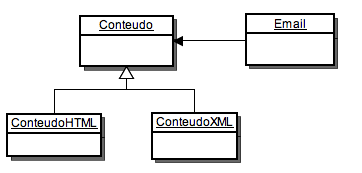
\includegraphics[scale=0.7]{imagens/email.png}
\par\end{centering}

\caption{Design que respeita o Princípio da Responsabilidade Única \label{img:email}}

\end{figure}

\subsubsection{Coesão}
De um ponto de vista técnico, qual crítica poderia ser feita sobre a classe \textit{Controlador}? 
A classe \textit{Controlador} não é coesa. Se tal classe tem a responsabilidade de lidar com a criação de HTML, logicamente terá um conjunto de variáveis de instância e métodos que as utilizam capazes de executar o trabalho em conjunto. O mesmo pode ser dito para o processamento da entrada do usuário. Um leitor que precisa entender apenas um desses contextos se deparará com inúmeros detalhes de implementação tanto da responsabilidade que deseja trabalhar, quanto da que não está interessado.
	
Quando a coesão de uma classe é alta, seus métodos e variáveis são codependentes e se unem como uma unidade lógica \citep{Beck2007}.De maneira mais prática, uma classe é totalmente coesa quando todos os seus métodos usam todas as variáveis de instância.
	
Dessa forma, a coesão da classe está intimamente relacionada com as responsabilidades que assume. Se uma classe tem muitas 
responsabilidades, provavelmente terá um conjunto de métodos que pouco se comunicam e usam poucas variáveis em comum, tendo baixa 
coesão. Quando a coesão é baixa, provavelmente será uma boa ideia criar uma nova classe.

Um bom exemplo de classe extremamente coesa é a implementação de uma estrutura de dados e suas operações. Na implementação 
simplificada de uma pilha apresentada abaixo, é fácil perceber como os métodos da classe \textit{Pilha} estão intimamente 
relacionados com suas variáveis de instância.

\lstinputlisting[label=pilha, caption={Classe coesa que implementa uma pilha}]{codigos/pilha}

\subsection{Acoplamento entre Classes}
Outro aspecto muito relevante do ponto de vista da orientação a objetos é o acoplamento entre as classes. Essa medida 
está atrelada a quanto as classes do sistema dependem uma das outras. As dependências podem se expressar de diversas 
formas desde o uso de um método de outra classe até a ``perigosa'' manipulação e modificação de dados de outra classe.
	
Tendo em vista a busca por consequências locais e a simplicidade e expressividade do código, não queremos que as 
classes dependam fortemente umas das outras de forma que o entendimento e a modificação de uma leve a alterações em 
outras classes. Além disso, a cada dependência gerada, os testes unitários criados provavelmente precisaram da 
utilização de artifícios para isolar cada uma das partes sendo mais difíceis de serem compreendidos.

Por outro lado, buscamos um sistema formado por muitas classes coesas e com uma única responsabilidade, fazendo com a comunicação 
entre os objeto seja inevitável. Diante desse cenário, o objetivo passa a ser a detecção de acoplamentos desnecessários, visando 
simplificar a comunicação entre os objetos através de suas interfaces.

Como vimos no exemplo da figura \ref{img:email}, uma solução encontrada para o problema foi criar uma depedência entre \textit{Email} 
com \textit{Conteudo}. O acoplamento criado não deixou as classes mais complexas, mas flexibilizou a criação de novas formatações.

Abaixo estão apresentados alguns conceitos e técnicas relacionados ao acoplamento em um código limpo.

\subsubsection{A Lei de Demeter (The Law of Demeter)}
A Lei de Demeter (\textit{The Law of Demeter}) diz que um método ``M'' de uma classe ``C'' só deveria chamar um dos 
seguintes métodos:

\begin{itemize}
	\item da própria classe;
	\item de um objeto criado por M;
	\item de um objeto passado como argumento para M;
	\item de um objeto guardado em uma variável de instância de C.
\end{itemize}

O cumprimento dessa heurística visa evitar que uma classe conheça os detalhes de implementação dos objetos aos quais 
manipula. A invocação de métodos da própria classe não causa nenhum tipo de dependência pela óbvia ausência de algo 
sobre a qual depender. Os outros tipos de chamadas especificados na Lei causam uma dependência, mas que se limita as 
interfaces dos objetos trabalhados. A classe deve conhecer quais os métodos dos objetos, os argumentos que aceitam e o 
tipo do valor de retorno, caso houver.
	
Um exemplo claro de violação são os chamados ``train wreck''. Suponha que temos uma classe \textit{JogoDeFutebol} e uma classe 
cliente ``C'' executa a seguinte operação:
	
\lstinputlisting[label=train_wreck, caption={Um chamado ``train wreck'' que exemplifica uma violação à Lei de 
Demeter}]{codigos/train_wreck}

A chamada para \textit{getTimes()} está de acordo com a Lei de Demeter, pois é uma invocação de um método de um objeto guardado em um 
variável de instância \textit{jogoDeFutebol} da classe \textit{JogoDeFutebol}. O valor de retorno dessa chamada é uma lista contendo 
os dois times que não é objeto criado e/ou guardado dentro da classe ``C'', nem um argumento passado para ``M''. Dessa forma, a 
chamada para \textit{primeiro()} sobre essa lista é a primeira das violações à heurística.
	
Considerando os problemas dessa abordagem e o acoplamento gerado, que partes do sistema a classe ``C'' conhece? Primeiramente, 
conhece a classe \textit{JogoDeFutebol}, já que possui um destes objetos guardados em uma variável de instância e chama um método 
\textit{getTimes()}. Além disso, conhece o valor de retorno desta chamada e sabe que é uma lista composta por objetos da classe 
\textit{Time} e que, portanto, poderia chamar o método \textit{primeiro()} sobre a lista. Ainda conhece que um Time tem uma coleção 
de cartões acessada através de \textit{getCartões()}, que aceita a mensagem \textit{count()}.
	
Esse exemplo mostra bem que tipo de problemas podem ocorrer quando acoplamento entre as partes do sistema está alta. Claramente, a 
classe ``C'' conhece muitas partes do sistema e, a partir desse momento, qualquer mudança nessa estrutura pode quebrar seu código. 
Quando temos que criar estruturas como a exemplificada, é necessário repensar o design e nos perguntarmos porque a classe ``C'' 
precisava ter acesso a todas aquelas informações. Provavelmente, é o caso de fazer mais delegações ao invés de depender tanto dos 
dados de outros objetos.

\subsubsection{Métodos ``Invejosos''}
Em alguns casos, um método mesmo sem violar a Lei de Demeter, tem um grande acoplamento com outra classe.
O exemplo abaixo não viola a Lei de Demeter, já que faz chamadas somente a métodos de um objeto que lhe foi passado como parâmetro.

\lstinputlisting[label=envy, caption={Método salario() é muito acoplado a classe Empregado sem violar a Lei de 
Demeter}]{codigos/envy}

O método \textit{salario} possui um grande acoplamento com a classe \textit{Empregado} ao utilizar diversos de seus métodos, de forma 
que ``inveja'' os seus dados \citep{Fowler99}.

\subsubsection{Delegação de Tarefa}
Para minimizar o acoplamento gerado pelos ``train wrecks'' e métodos ``invejosos'', temos que considerar uma mudança nas 
tarefas realizadas pelas classes envolvidas. Se um método da classe ``A'' utiliza muitos métodos e dados da classe ``B'', muito 
provavelmente sua tarefa pertence a ``B'' já que queremos aproximar a lógica e seus dados.

Dessa maneira, uma possível solução consiste na alteração do método para que ``peça'' a classe ``B'' para que realize uma tarefa 
através de um novo método. Podemos dizer que o método fez uma ``Delegação de Tarefa''.

O exemplo abaixo ilustra métodos de uma classe \textit{CalculaReceita}, cujo código poderia se beneficiar com uma Delegação de Tarefa.

\lstinputlisting[label=pedido_de_tarefa, caption={Método salarioDoMes com problemas de ``inveja''}]{codigos/pedido_de_tarefa}

Claramente o método \textit{salarioDoMes} tem problemas de ``inveja'' sobre a classe \textit{Empregado}. Podemos observar algumas mudanças 
importantes: (i) o método \textit{calculaTotalDeSalarios} ficou muito simples só fazendo um Delegação de Tarefa para a classe \textit{Empregado}; 
(ii) o código do método \textit{salarioDoMes} também ficou mais simples já que foi transferido para perto dos dados que utiliza; (iii) de forma 
geral, reduzimos o acoplamento entre as classes pois existe apenas uma chamada de método para fazer a comunicação.

\lstinputlisting[label=pedido_de_tarefa2, caption={Redução entre o acoplamento das classes CalculaReceita e Empregado}]{codigos/pedido_de_tarefa2}

\subsubsection{Objeto Centralizador}
Os cenários apresentados acima consideram que uma classe depende somente de uma segunda. No entanto, frequentemente criamos métodos 
que lidam com mais de uma classe, gerando um grande acoplamento entre as envolvidas.

Associada com o objetivo de minimização de dependências e a criação de classes com única responsabilidade, uma 
maneira de contornar esse cenário é criar uma classe que possa fazer essa relação entre classes. De maneira 
bastante análoga ao desenvolvimento do Objeto Método 
(\ref{objeto_metodo}), o intuito é transferir a atividade complexa de centralizar a comunicação entre objetos 
diferentes para um novo ``objeto centralizador''.

São dois resultados importantes dessa alteração: (i) isolaremos a complexidade do acoplamento entre classes em uma classe que poderá receber testes e refatorações independentes; (ii) a medida que encapsulamos as dependências entre objetos, obtemos mais classes que podem ser mais facilmente reaproveitadas posteriormente.

\subsubsection{Princípio da Inversão de Dependência (Dependency Inversion Principle)}
O objetivo da minimização do acoplamento entre nossas classes é facilitar as alterações que serão feitas no sistema. Queremos conseguir estender a infra-estrutura de classes que temos para criar novas funcionalidades.
	
No exemplo utilizado por Robert Martin em sua coluna para a revista \textit{The C++ Report}
sobre o assunto discutido, temos uma classe  \textit{Copiador} que utiliza um \textit{LeitorDeTeclado} para coletar inteiros digitados pelo usuário e um  \textit{EscritorDeArquivo} para escrever o dado em um arquivo. Quais alterações precisam ser feitas  para adicionar a funcionalidade de ler os inteiros de um arquivo? Será necessário criar mudanças na classe  \textit{Copiador} para que possa receber dados coletados de dois tipos diferentes de objetos que lidam com a entrada de dados. Tal alteração só se torna necessária devido a dependência que Copiador tem com classes como \textit{EscritorDeArquivos} e \textit{LeitorDoTeclado}.
	
A solução ideal para o problema seria que  \textit{Copiador} dependesse de abstrações como \textit{Leitor} e  \textit{Escritor} que tivesse uma interface definida de forma que subclasses como  \textit{LeitorDeTeclado} ou  \textit{LeitorDeArquivo} pudessem ser utilizadas polimorficamente. Todos os tipos de  \textit{Leitor} teriam que seguir uma abstração ao implementar o método  \textit{lerInteiro()} e  \textit{Copiador} só precisaria depender dessa interface. Essa mudança seguiria o Princípio da Inversão de Dependência (\textit{Dependency Inversion Principle} \citep{Martin97c}) , que diz:
	
\begin{itemize}
 	\item Classes de alto nível não devem depender de classes de baixo nível. Ambas deveriam depender de abstrações.
	\item Abstrações não devem depender de detalhes. Detalhes devem depender de abstrações.
\end{itemize}

Durante o desenvolvimento, frequentemente essa solução pode não ser clara ou, em um cenário oposto, os programadores tentam prever todas as partes do código que enfrentam esse problema e utilizam a Inversão de Dependência. Entretanto, nenhum dos casos pode ser o ideal para o código. Como afirmado por Kent Beck ~\citep{Beck2007}, só devemos investir em flexibilidade em partes do sistema que realmente precisam de flexibilidade. Dessa forma, talvez a melhor solução não precise ser implementada em um primeiro momento, mas quando a necessidade surgir. Provavelmente, nesse instante temos que ter certeza que fizemos uma boa escolha para as próximas alterações.

Outro fato importante a ser considerado quanto a Inversão de Dependência está no isolamento dos testes automatizados. Ao testar classes que dependem de outras classes, queremos isolar a testada de forma que os testes sejam de fato unitários. Se a classe em teste depender de abstrações, o trabalho será simplificado. No exemplo da classe \textit{Copiador}, poderíamos criar um \textit{EscritorTeste} e um \textit{LeitorTeste} que tivesse operações convenientes para que os testes de \textit{Copiador} fosse isolados.


\section{Unindo Conceitos}
\label{unindo_conceitos}
Nas sessões anteriores foram enumeradas diversas características que devem ser consideradas para o desenvolvimento de 
um código limpo. Através de uma parcela do conjunto apresentado, podemos fazer boas escolhas que trarão melhorias 
imediatas para o código. Entretanto, o entendimento e aplicações de composições das recomendações podem causar 
alterações ainda mais poderosas.

Para exemplificar a união dos conceitos apresentados ao longo capítulo, apresentaremos a seguir um 
conjunto de melhorias para o código de uma classe \textit{Digrafo} que implementa uma lista de adjacência para 
representar as arestas de um grafo dirigido, além de calcular a árvore geradora de custo mínimo através do algoritmo de 
Dijkstra no método \textit{custosAPartirDoVertice}.

Inicialmente, a classe se comunica com duas classes: \textit{Aresta} representa uma ligação de um vértice com outro e o 
custo desta ligação, enquanto que \textit{FilaDePrioridade} representa uma uma fila com prioridades com as operações 
\textit{vazia()}, \textit{insere(aresta)} e \textit{verticeDaArestaComCustoMinimo()}.

\lstinputlisting[label=digrafo1, caption={Classe Digrafo com problemas de limpeza}]{codigos/digrafo/digrafo1}

O problema mais aparente desse código é a complexidade do método \textit{custosAPartirDoVertice}. Um leitor 
que não conhece o algoritmo teria grandes dificuldades para compreender sua implementação devido a falta de 
expressividade do método. São muitas linhas de código, diversos detalhes de implementação e estruturas encadeadas 
complexas para realizar muitas tarefas. 

A primeira alteração que pode ser feita é a criação de Métodos como Condicionais (\ref{metodos:condicionais}) e 
Métodos Explicativos (\ref{metodos:explicativos}) para auxiliar a responder questões sobre algumas operações.

Por exemplo, o que significa a expressão booleana \textit{custos[verticeDestino] == -1}? Em uma visão mais detalhada, 
podemos observar que os custos de todos os vértices foram inicialmente inicializados com a constante ``-1'', 
representando que, até momento, o vértice não foi atingido e não sabemos quanto custa um caminho até ele. Uma solução 
interessante capaz de gerar uma maior clareza e documentação da implementação é a criação dos métodos abaixo
exibidos.

\lstinputlisting[label=metodos_explicativos, caption={Métodos Explicativos}]{codigos/digrafo/nao_atingido}

Além da criação de métodos com a mesma motivação, poderemos também quebrar as etapas do algoritmo através da Composição 
de Métodos (\ref{metodos:composicao}). Essa mudança se baseia no desenvolvimento de um conjunto de métodos com nomes 
significativos para encapsular operações em diferentes níveis de abstração, além de minimizar as estruturas encadeadas.
O trecho de código abaixo mostra um método \textit{inicializaCustos} criado para encapsular a inicialização do vetor de 
custos.

\lstinputlisting[label=inicializa_custos, caption={Processo de inicialização do vetor de custos fica mais claro com a Composição de Métodos}]{codigos/digrafo/inicializa_custos}

Toda inicialização do vetor de custos fica mais clara através desse método. Operações confusas como 
\textit{custos[vertice] = 0} agora se encontram encapsuladas e com um nome explicativo.

Podemos observar que a contínua aplicação da Composição de Métodos gera um crescimento no número de métodos e no total de 
linhas da classe, mas cada um dos métodos possui poucas linhas de código e realiza apenas uma tarefa simples e direta. 
Outra consequência é a necessidade da passagem de argumentos como \textit{custos} e \textit{fila}, uma vez que os métodos 
de menor nível de abstração são aqueles que efetivamente realizam as operações utilizando-os.

Para solucionar esse aumento no número de argumentos sendo repassados através da classe, podemos promover alguns destes à 
variáveis de instância (\ref{metodos:parametros}). É fácil notar nos exemplos abaixo como essa alteração limpa o código 
dos métodos de mais alto nível que não utilizam os argumentos em suas tarefas.

\lstinputlisting[label=sem_argumentos, caption={Métodos de alto nível sem a passagem de argumentos}]{codigos/digrafo/sem_argumentos}

Todas as alterações feitas até o momento foram feitas levando em conta a melhoria do código dos métodos que compõe a 
classe \textit{Digrafo}. Porém uma grande alteração podería ser feita ao levar a abstração encapsulada sobre essa classe.
Por quais motivos poderia ser alterada? Primeiramente, poderia ser mudada caso fosse necessário implementar o grafo 
dirigido com uma matriz de adjacência ao invés de uma lista. Também poderiamos querer alterar o algoritmo de Dijkstra 
para utilizar outra alternativa.

Claramente a classe \textit{Digrafo} viola o Princípio da Única Responsabilidade. De um ponto de vista mais técnico, 
podemos observar que as variáveis de instância \textit{custo} e \textit{fila} não são utilizadas pelos métodos 
\textit{adicionaAresta} e \textit{arestaDoVértice}, mas só são de interesse dos métodos desenvolvidos para a composição 
do método \textit{custosAPartirDoVertice}.

A solução para essa falta de coesão é a divisão em duas classes. Essa ruptura poderia ser feita de forma a preservar o 
método \textit{custosAPartirDoVertice} na interface \textit{Digrafo}, implementando o método através da delegação para 
uma nova classe que encapsula o algoritmo. No entanto, essa decisão causaria uma dependência circular: \textit{Digrafo} 
dependeria da nova classe \textit{CalculadorDijkstra} para calcular a árvore geradora de custo mínimo e, por outro lado,
\textit{CalculadorDijkstra} dependeria das arestas e vértices de \textit{Digrafo}.

Uma solução mais interessante é \textit{CalculadorDijkstra} receber como argumento de seu construtor um objeto \textit{Digrafo}. Dessa maneira, a classe \textit{Digrafo} ficou pequena e coesa com a única responsabilidade de criar a representação do grafo.

\lstinputlisting[label=digrafo_final, caption={Classe Digrafo com apenas uma responsabilidade}]{codigos/digrafo/digrafo_final}
 
O resultado do esforço exemplificado é um conjunto de classes que atingiu grande proximidade para com os três valores: 
expressividade, simplicidade e flexibilidade.
O código ficou significantemente mais expressivo, pois as classes são formadas por muitos métodos com bons nomes de forma que o leitor possa ler cada nível de abstração em uma linguagem bastante próxima da natural.
 
Além disso, a composição com classes pequenas e extremamente coesas torna mais simples a compreensão de cada uma das partes, uma vez que é necessário trabalhar com pouca informação para entender um método ou uma classe. Se essas características também forem empregadas para as outras classes do sistema, resultam na minimização de duplicações, na aproximação da lógica e dados e na manutenção de consequências locais, provendo maior flexibilidade.

A tabela abaixo resume as técnicas apresentadas ao longo do capítulo.

\newenvironment{my_itemize}
{\begin{list}{\labelitemi}
{  \setlength{\itemsep}{0pt}
  \setlength{\parskip}{0pt}
  \setlength{\parsep}{0pt}
  \setlength{\topsep}{0pt}
  \setlength{\partopsep}{0pt}
  \setlength{\leftmargin}{1em}
  \setlength{\rightmargin}{0.5em}
  \setlength{\topmargin}{0.5em}
}
}
{\end{list}}    
     

\begin{landscape}

\begin{table}[hbt]

\scalefont{.85}
\begin{tabular}{|p{3.5cm}|p{5cm}|p{8.5cm}|p{7.2cm}|}
\hline 
\textbf{Técnica} & \textbf{Descrição} & \textbf{Contribuições} & \textbf{Consequências} \tabularnewline
\hline

\hline 
Composição de Métodos 
& Compor os métodos em chamadas para outros rigorosamente no mesmo nível de abstração abaixo
& \begin{my_itemize}
	\item Facilidade de entendimento de métodos menores
	\item Criação de métodos menores com nomes explicativos
  \end{my_itemize}
& \begin{my_itemize}
	\item[-] Operações por métodos
	\item[+] Número de parâmetros da classe
	\item[+] Métodos na classe
  \end{my_itemize}
\tabularnewline

\hline 
Métodos Explicativos
& Criar um método que encapsule uma operação pouco clara geralmente associada a um comentário
& \begin{my_itemize}
	\item O código cliente do método novo terá uma operação com nome que melhor se encaixa no contexto
  \end{my_itemize}
& \begin{my_itemize}
	\item[+] Métodos na classe
  \end{my_itemize}
\tabularnewline

\hline 
Métodos como Condicionais
& Criar um método que encapsule uma expressão booleana para obter condicionais mais claros
& \begin{my_itemize}
	\item Facilidade na leitura de condicionais no código cliente
	\item Encapsulamento de uma expressão booleana	
  \end{my_itemize}
& \begin{my_itemize}
	\item[+] Métodos na classe
  \end{my_itemize}
\tabularnewline

\hline 
Evitar Estruturas Encadeadas
& Utilizar a composição de métodos para minimizar a quantidade de estruturas encadeadas em cada método
& \begin{my_itemize}
	\item Facilidade para a criação de testes
	\item Cada método terá estruturas mais simples e fáceis de serem compreendidas
  \end{my_itemize}
& \begin{my_itemize}
	\item[-] Estruturas encadeadas por método (o número total da classe continuará inalterado)
  \end{my_itemize}
\tabularnewline

\hline 
Cláusulas Guarda
& Criar um retorno logo no inicio de um método ao invés da criação de estruturas encadeadas com if sem else
& \begin{my_itemize}
	\item Estruturas de condicionais mais simples
	\item Leitor não espera por uma contrapartida do condicional(ex: if sem else)
  \end{my_itemize}
& \begin{my_itemize}
	\item[-] Estruturas encadeadas na classe
  \end{my_itemize}
\tabularnewline

\hline
Objeto Método
& Criar uma classe que encapsule uma operação complexa simplificando a original (cliente)
& \begin{my_itemize}
	\item O código cliente terá um método bastante simples
	\item Nova classe poderá ser refatorada sem preocupações com alterações no código cliente
	\item Nova classe poderá ter testes separados
  \end{my_itemize}
& \begin{my_itemize}
	\item[-] Operações no método cliente
	\item[-] Responsabilidades da classe cliente
	\item[+] Classes
	\item[+] Acoplamento da classe cliente com a nova classe
  \end{my_itemize}
\tabularnewline

\hline
Evitar Flags como Argumentos
& Ao invés de criar um método que recebe uma flag e tem diversos comportamentos, criar  um  método para cada comportamento
& \begin{my_itemize}
	\item Leitor não precisará entender um método com muitos condicionais
	\item Testes unitários independentes
  \end{my_itemize}
& \begin{my_itemize}
	\item[+] Métodos na classe
  \end{my_itemize}
\tabularnewline

\hline
\end{tabular}
\caption{Parte I - Técnicas: descrição, contribuições e consequências}
\scalefont{1}
\end{table}


\begin{table}[hbt]
\scalefont{.85}
\begin{tabular}{|p{3.5cm}|p{5cm}|p{8.5cm}|p{7.2cm}|}
\hline 
\textbf{Técnica} & \textbf{Descrição} & \textbf{Contribuições} & \textbf{Consequências} \tabularnewline
\hline

\hline
Objeto como Parâmetro
& Localizar parâmetros que formam uma unidade e criar uma classe que os encapsule
& \begin{my_itemize}
	\item Menor número de parâmetros facilita testes e legibilidade
	\item Criação de uma classe que poderá ser reutilizada em outras partes do sistema
  \end{my_itemize}
& \begin{my_itemize}
	\item[-] Parâmetros passados pela classe
	\item[+] Classes
	\item[+] Acoplamento da classe cliente com a nova classe
  \end{my_itemize}
\tabularnewline

\hline
Parâmetros como Variável de Instância
& Localizar parâmetro muito utilizado pelos métodos de uma classe e transformá-lo em variável de instância
& \begin{my_itemize}
	\item Não haverá a necessidade de passar longas listas de parâmetros através de todos os métodos
  \end{my_itemize}
& \begin{my_itemize}
	\item[-] Parâmetros passados pela classe
	\item[-] Possível diminuição na coesão
  \end{my_itemize}
\tabularnewline

\hline
Uso de Exceções
& Criar um fluxo normal separado do fluxo de tratamento de erros utilizando exceções ao invés de valores de retornos e condicionais
& \begin{my_itemize}
	\item Clareza do fluxo normal sem tratamento de erros através de valores de retornos e condicionais
  \end{my_itemize}
& \begin{my_itemize}
	\item[-] Estruturas Encadeadas
  \end{my_itemize}
\tabularnewline

\hline
Maximizar Coesão
& Quebrar uma classe que não segue o Princípio da Responsabilidade Única
& \begin{my_itemize}
	\item Cada classe terá uma única responsabilidade
	\item Cada classe terá seus testes independentes
	\item Sem interferências na implementação das responsabilidades
  \end{my_itemize}
& \begin{my_itemize}
	\item[+] Classes
	\item[-] Métodos em cada classe
	\item[-] Atributos em cada classe
  \end{my_itemize}
\tabularnewline

\hline
Delegação de Tarefa
& Transferir um método que utiliza dados de uma classe ``B'' para a ``B'' 
& \begin{my_itemize}
	\item Redução do acoplamento entre as classes
	\item Proximidade dos métodos e dados sobre os quais trabalham
  \end{my_itemize}
& \begin{my_itemize}
	\item[-] Métodos na classe inicial
	\item[+] Métodos na classe que recebe o novo método
  \end{my_itemize}
\tabularnewline

\hline
Objeto Centralizador
& Criar uma classe que encapsule uma operação com alta dependência entre classes
& \begin{my_itemize}
	\item Simplificação da classe cliente
	\item Redução do acoplamento da classe cliente com as demais
	\item Nova classe poderá receber testes e melhorias independentes
  \end{my_itemize}
& \begin{my_itemize}
	\item[-] Operações no método cliente
	\item[-] Responsabilidades da classe cliente
	\item[+] Classes
	\item[+] Acoplamento da classe cliente com a nova classe
  \end{my_itemize}
\tabularnewline
\hline
\end{tabular}

\caption{Parte II - Técnicas: descrição, contribuições e consequências}
\scalefont{1}
\end{table}

\end{landscape}

